\documentclass[12pt]{article}
\usepackage[left=2cm,right=2cm,top=2cm,bottom=2cm]{geometry}
\usepackage{wrapfig}
\usepackage{booktabs}
\usepackage{graphicx}
\usepackage{amssymb} 
\usepackage{siunitx} % Required for alignment
\usepackage{subfigure}
\usepackage{multirow}
\usepackage{rotating}
\usepackage[T2A]{fontenc}
\usepackage[english, russian]{babel}
\usepackage{caption}
\usepackage{hyperref}
\usepackage{mathtools}
\usepackage{amsmath}
\usepackage{float}

\hypersetup{
    colorlinks=true,
    linkcolor=red,
    urlcolor=magenta,
    }
\graphicspath{{pictures/}}

\begin{document}
    \begin{titlepage}
        \begin{center}
            \vspace*{1cm}

            \Huge
            \textbf{ИЗМЕРЕНИЕ ТЕПЛОПРОВОДНОСТИ ВОЗДУХА ПРИ РАЗНЫХ ДАВЛЕНИЯХ}

            \vspace{1.5cm}

            \Large
            \textbf{Комкин Михаил Б01-303}

            \vfill

            Вопрос по выбору \\
            Устный экзамен по общей физике

            \vspace{0.8cm}

            
\includegraphics[width=0.4\textwidth]{university_logo.png}

            Физтех-школа радиотехники и компьютерных технологий\\
            Московский физико-технический институт\\
            Долгопрудный, 2024
        \end{center}
    \end{titlepage}
    
    \begin{itemize}
        \item{Цель работы:} исследовать теплопередачу от нагретой нити к цилиндрической оболочке в зависимости от концентрации\\ 
        (давления) заполняющего её воздуха. Измерить коэффициент теплопроводности при высоких давлениях; определить область перехода к 
        режиму теплопередачи; определить коэффициент теплопередачи при низких давлениях.\\
        \item{В работе используются:} цилиндрическая колба с натянутой по оси платиновой нитью; форвакуумный насос; вакуумметр; масляный манометр; вольтметр и амперметр
        (цифровые мультиметры); источник постоянного тока.
    \end{itemize}
    \section{Теоретические сведения}  
        \textbf{Теплопроводность} — это процесс передачи энергии от нагретых частей атомов и т.п.). В газах теплопроводность осуществляется за 
        счёт непосредственной передачи кинетической энергии от быстрых молекул к медленных при их столкновениях. Перенос тепла 
        описывается \textbf{законом Фурье} - плотность потока энергии $\vec{q}$ пропроциональна граденту температуры $\nabla T$
        \begin{equation}\label{зн Фурье}
            \vec{q} = - \varkappa \nabla T
        \end{equation}
        Коэффициент $\varkappa$ - \textbf{коэффициент теплопроводности}. В данной работе система имеет цилиндрическую симметрию, принебрегая краевыми эффектами,
        можно считать, что все параметры газа зависят только от расстояния до оси системы $r$. Тогда вместо \ref{зн Фурье} имеем:
        \begin{equation}
            q = - \varkappa \frac{dT}{dr}
        \end{equation}
        Система, в которой имеюстся перепады температур, не находитсяв состоянии равновесия. Говоря о зависимости температуры от координат $T(r)$ мы подразумеваем, что систему
        можно разбивать на элементарные подсистемы(малые объемы), в каждой из которых имеет место локальное тепловое равновесие. В газах 
        закон Фурье применим, если характерный размер $r$ задачи превосходит длину свободного пробега молекул: $\lambda << r$, а температуры меняется незначительно на масштабах 
        длины пробега: $\lambda|\nabla T| << T$.\\
        Для количественного описания способности некоторой системы к теплопередач в целом используют коэффициент, называемый температурным сопротивлением, 
        равный отношению перепада температур $\Delta T$ в системе к полному потоку энергии $Q$ через нее:
        \begin{equation}\label{q = }
            K = \frac{\Delta T}{Q}
        \end{equation}\\
        \textbf{Плотные газы} В условиях применимости закона Фурье дадим оценку коэффициенту теплопроводности.\\
        Принимается, что вдоль каждой из осей координат (X,Y,Z) движется по 1/3 всех молекул, 1/6 — в положительном 
        и 1/6 — в отрицательном направлениях.\\
        \begin{figure}[H]
            \centering
            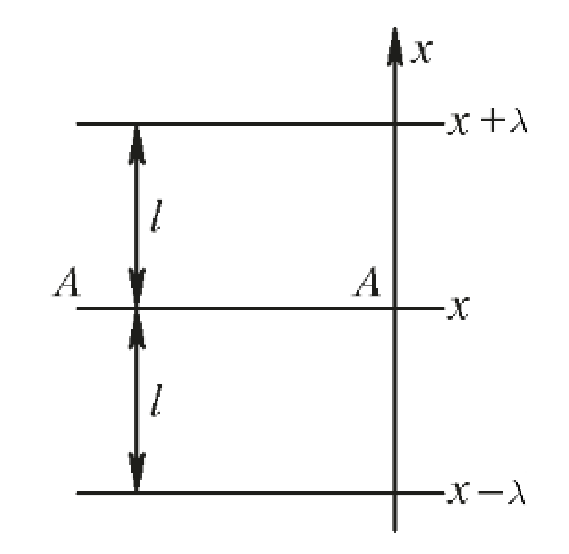
\includegraphics[width=0.4\linewidth]{furie_image.png}
            \caption{К определению коэффициентов переноса}
            \label{fig:mpr}
        \end{figure}
        Рассмотрим движение молекул вдоль оси $x$. Число молекул, проходящих вверх за время свободного пробега $\tau$ через
        единицу площади в плоскости с координатой $x$, равно
        \[ N^{(\uparrow)} = \frac{1}{6}n(x-\lambda) \vec{v} \tau \]           
        \[ N^{(\downarrow)} = \frac{1}{6}n(x+\lambda) \vec{v} \tau \]
        Здесь $\vec{v}$ — средняя тепловая скорость, а $l$ — длина свободного пробега молекулы.\\
        Будем считать, что перемещения газа как целого вдоль оси $x$ нет. Это значит, что $N^{(\uparrow)} =  N^{(\downarrow)}$.
        Пусть $\eta(x) = c_v$ $T(x)$ — энергия молекулы в точке $x$, $c_v$ — теплоемкость, приходящаяся на одну молекулу. 
        Тогда согласно определению теплового потока.
        \[
            q = \frac{\eta(x-\lambda)N^{(\uparrow)} - \eta(x+\lambda)N^{(\downarrow)}}{\tau}
        \]
        Отсюда следует 
        \begin{equation}\label{kappa}
            \varkappa = \frac{1}{3} n \vec{v}lc_v 
        \end{equation}
        где $n$ - концентрация молекул газа, $\vec{v} = \sqrt{\frac{8RT}{\pi\mu}}$ - их средняя тепловая скорость,
        $c_v = \frac{i}{2}k_{\text{Б}}$ - теплоемкость при постоянном объеме в расчете на одну молекулу.\\
        Длина свободного пробега обратно пропорциональна $n$: $\lambda = \frac{1}{n\sigma}$ (где$\sigma$ — эффективное 
        сечение столкновений молекул друг с другом), поэтому коэффициент теплопроводности газа \ref{kappa} не зависит от его 
        концентрации (а значит, и от давления) и определяется только его температурой.

        \textbf{Разреженные газы}\\
         Пусть газ разрежен настолько, что длина свободного пробега молекул относительно столкновений друг 
        с другом $\lambda = \frac{1}{n\sigma}$ превосходит характерные размеры системы: $r \gtrsim \lambda$. Тогда молекулы 
        сталкиваются в основном не между собой, а со стенками. При этом теряет смысл понятие
        температуры как функции координат и, следовательно, градиента температуры, так что закон Фурье \ref{зн Фурье} 
        становится неприменим. Если в системе есть поверхности, находящиеся при разных температурах, процесс обмена энергией 
        между ними за счёт молекул газа, заполняющего сосуд, принято называть теплопередачей (возможен также теплообмен за счёт излучения). Молекулы 
        при неупругих ударах о нагретую поверхность приобретают среднюю
        кинетическую энергию, соответствующую температуре этой поверхности;
        отразившись от неё и не сталкиваясь с другими молекулами, они долетают до
        холодной поверхности и передают ей избыточную энергию. Отметим, что такое состояние газа является неравновесным, поэтому
        температура самого газа, строго говоря, не определена.\\
        \textbf{Теплопередача в разреженном газе}\\
        \begin{figure}[H]
            \centering
            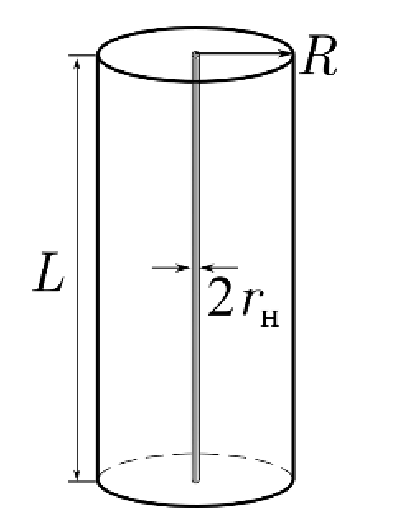
\includegraphics[width=0.4\linewidth]{task_geometry.png}
            \caption{К определению коэффициентов переноса}
            \label{fig:mpr}
        \end{figure}
        Рассмотрим упрощённую модель теплопередачи в цилиндрическом сосуде радиуса $R$ и длины $L$ ($L >>R$),
        на оси которого натянута тонкая нить радиуса $r_\text{н}$ ($r_\text{н} << R$), см $\ref{task_geometry.png}$
        Пусть температуры колбы и нити равны $T_\text{к}$ и $T_\text{н}$ соответственно ($T_\text{н}$ > $T_k$). 
        Предположим сначала, что длина свободного пробега превосходит радиус колбы $\lambda \gtrsim R$.
        Все молекулы в пространстве колбы можно разделить на две группы: в зависимости от того, с какой поверхноcтью — 
        с колбой или с нитью — они испытали последнее неупругое столкновение, их средняя энергия равна $c_vT_\text{к}$ либо $c_vT_\text{н}$
        соответственно. В стационарном состоянии потоки частиц, падающих на нить и улетающих от неё, равны.\\
        Найдем полный поток частиц падающих на нить.
        \begin{figure}[H]
            \centering
            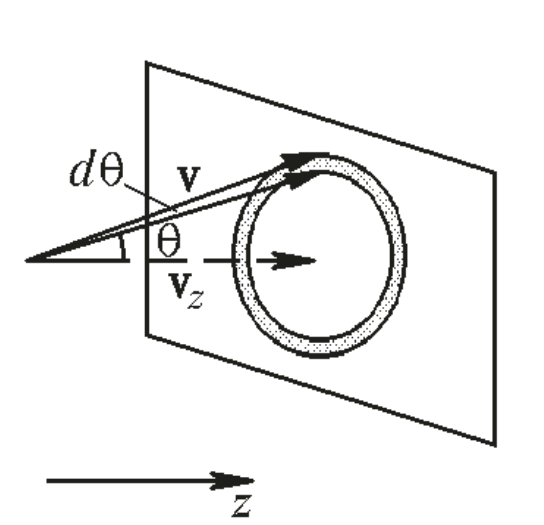
\includegraphics[width=0.4\linewidth]{collision_with_wall.png}
            \caption{К определению коэффициентов переноса}
            \label{collision}
        \end{figure}
        Рассмотрим столкновения молекул газа с неподвижной стенкой (\ref{collusion}). Выделим группу молекул, 
        имеющих скорость $v$. Плотность этих молекул обозначим $dn(v)$. Вследствие изотропии газа в телесный угол 
        $d\Omega = \pi sin(\theta d\theta)$ летит доля молекул, равная $d\Omega/(4\pi)$. Соответственно, 
        плотность этих молекул равна $dn(v)d\Omega/(4\pi)$. За время $dt$ до поверхности долетят молекулы, удаленные 
        от нее на расстояние $v_zdt$, где $v_z = v cos\theta$. Всего в площадку $dS$ попадут молекулы, находящиеся в 
        цилиндре объемом $v_zdtdS$, содержащем $v_zdtdSdn(v)d\theta/(4\pi)$ молекул выделенной группы. Суммируя результат 
        по всем допустимым углам $(0 < \theta < \pi/2)$ и скоростям $(0 < v < \infty)$ и деля результат на $dtdS$, получаем
        \begin{equation}
            \int\limits vcos\theta\frac{d\Omega}{4\pi}\,dn(v) = n\int\limits_0^\infty n\Phi(v)\,dv \frac{1}{4\pi}\int\limits_0^\frac{\pi}{2} cos\theta 2\pi sin\theta\,d\theta = \frac{1}{4}n\vec{v}
        \end{equation}
        Полный поток будет составлять
        \[
            J = jS = \frac{1}{4}n\vec{v}S_{\text{н}}
        \]  
        где $n$ — концентрация частиц, $\vec{v}$ — их средняя тепловая скорость, $S_\text{н} = 2\pi r_{\text{н}L}$ — площадь поверхности нити. 
        В нашей работе относительный перепад температур мал, $\Delta T << T_\text{к}$, поэтому при расчёте потока частиц можно не
        различать средние скорости летящих от нити и летящих к нити частиц. Учтём, что не все столкновения молекул с нитью или 
        стенками колбы являются неупругими (при упругом отражении молекула не передаёт энергию
        стенке). Для этого введём поправочный множитель $s$, называемый коэффициентом аккомодации. Он пропорционален вероятности неупругого удара,
        которая определяется структурой и материалом поверхности и, вообще говоря, может зависеть от $T$, однако при $\Delta T << T_{\text{к}}$ 
        его можно считать постоянным.\\
        Таким образом, суммарный поток энергии от нити к колбе может быть приближённо записан как
        \[
            Q \approx \frac{s}{4} n \vec{v} S_{\text{н}}c_v(T_\text{н}-T_{\text{к}}) 
        \]
        Отсюда получаем тепловое сопротивление системы в режиме теплопередачи:
        \begin{equation}\label{K}
            \frac{1}{K_{\text{т}} = \frac{s}{4} n \vec{v} S_{\text{н}}c_v}
        \end{equation}
        Важно, что в отличие от случая плотного газа, интенсивность теплопередачи зависит от концентрации газа в колбе $n$ $(T_{\text{к}} \propto 1/n)$. То есть, 
        при заданной мощности нагрева $Q$ приращение температуры нити $\Delta T = T_{\text{н}-T_{\text{к}}}$ будет
        меняться обратно пропорционально $n$. Отметим также сходство формул (\ref{kappa}) и (\ref{K}): видно, что с точностью до коэффициента порядка единицы
        \[
            \frac{1}{K_{\text{т}}} \sim \frac{r_{\text{н}}}{\lambda}\varkappa \sim r_{\text{н}}\vec{v}nc_v
        \]
        Таким образом, в сильно разреженном газе роль длины свободного пробега
        играет характерный размер задачи (в данном случае, радиус нити $r_{\text{н}}$). Стоит отметить, что как (\ref{kappa}), так и (\ref{K}), дают лишь оценки по порядку
        величины. При этом, однако, они правильно описывают функциональные зависимости от параметров газа (в частности, от концентрации), что позволяет
        определить значения неизвестных коэффициентов экспериментально.\\
        \textbf{Общий случай}
        \begin{figure}[H]
            \centering
            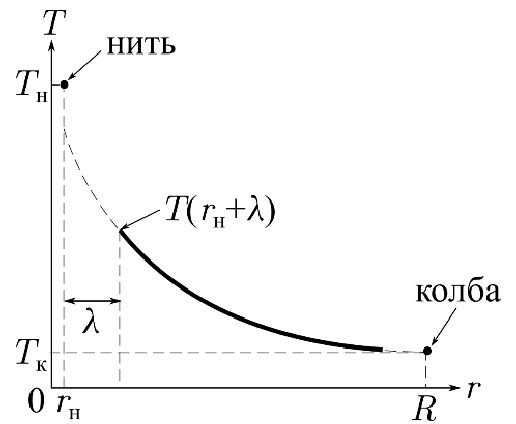
\includegraphics[width=0.4\linewidth]{system_tempetatute.png}
            \caption{температура системы}
            \label{fig:mpr}
        \end{figure}
        Рассмотрим теплообмен между нитью и стенками цилиндрической колбы при произвольных значениях концентрации газа.
        При больших $n$ длина свободного пробега много меньше диаметра нити, поэтому реализуется режим теплопроводности, в
        котором коэффициент теплопроводности $varkappa$ не зависит от $n$. С уменьшением давления в
        системе $P = nk_{\text{Б}}T$ пропорционально уменьшается и концентрация $n$, так что длина пробега может оказаться больше 
        радиуса нити: $r_{\text{н}} \lesssim \lambda << R$ (предел $\lambda \gtrsim R$ в установке не достигается). При этом вблизи нити появится 
        область теплопередачи размером $\sim \lambda$, в которой закон Фурье неприменим (см \ref{температура системы}).\\
        Стоит также отметить, что аналогичный участок имеется и вблизи поверхности колбы при $R - \lambda \le r \le R$, однако 
        его влиянием можно принебречь, посколько плотность потока энергии там мала, а следовательно мал и 
        градиент температуры: $\frac{dT}{dr}\bigg|_{r=R} << \frac{dT}{dr}\bigg|_{r=r_{\text{н}}} $\\
        Пусть через нить пропускат постоянный ток, так что на ней выделяется известная мощьность $Q$. В стационарном состоянии полный поток энергии через 
        любую цилиндрическую поверхность радиуса $r$ должен быть одинаков и равен $Q$. В области теплопроводности из (\ref{q =}) имеем
        \begin{equation}\label{Q}
            Q = -2\pi r L\varkappa \frac{dT}{dr} = const
        \end{equation}
        Если перепад температуры между стенками колбы и нитью мал ($\Delta T << T_{\text{к}}$), при интегрировании \ref{Q} можно принебречь зависимостью теплопроводности
        от температуры, положив $\varkappa \approx \varkappa(T_{\text{к}})$. Тогда получим 
        \begin{equation}\label{T_r)}
            T(r) - T_{\text{к}} = \frac{Q}{2\pi L\varkappa}ln \frac{R}{r}
        \end{equation}
        В области вблизи нити $r_{\text{н}} \le r \lesssim r_{\text{н}} + \lambda$ имеем
        \begin{equation}\label{T_h}
            T_{\text{н}} - T(r_{\text{к}} + \lambda) = K_{\text{т}}Q
        \end{equation}
        где $K_{\text{т}}$ — тепловое сопротивление области теплопередачи, определяемое формулой (\ref{K}), $T(r_{\text{н}} + \lambda)$ — температура газа на границе этой области. Подставив
        в (\ref{T_r}) $r = r_{\text{н}} + \lambda$ и, исключив с помощью (\ref{T_h}) промежуточную температуру $T(r_{\text{к}} + \lambda)$, найдём разность температур нити и колбы:
        \begin{equation}
            \Delta T = Q \left|\frac{1}{2\pi L \varkappa}ln\frac{R}{r_{\text{н}+\lambda}} + K_{\text{т}} \right|
        \end{equation}
        С учетом формул ДОБАВИТЬ ССЫЛКИ эту формулу можно переписать в виде:
        \begin{equation}\label{T}
            \Delta T = \frac{Q}{2\pi L}\left| \frac{1}{\varkappa}ln\frac{R}{r_{\text{н}}+\frac{1}{n\sigma}} +\frac{1}{\frac{s}{4} n \vec{v} S_{\text{н}}c_v} \frac{1}{n}\right|
        \end{equation}
        Можно упростить \ref{T} до вида 
        \begin{equation}
            \Delta T = Q \left|K_{\infty} + \frac{A}{P}\right|
        \end{equation}
        где 
        \[
            A = \frac{4}{s\vec{v}c_v}\frac{k_{\text{Б}}T}{S_H}
        \] 
        $K_{\infty}$ есть тепловое сопротивление системы при высоких давлениях,
        по его значению может быть вычислен коэффициент теплопроводности газа $\varkappa$. По значению коэффициента $A$ можно определить коэффициент
        аккомодации $s$ и таким образом найти тепловое сопротивление системы при любом давлении.
   
    \section{Установка}
        Схема установки приведена на \ref{vacuum_part}. Внутренняя полость тонкостенной
        цилиндрической стеклянной колбы, на оси которой натянута металлическая
        (платиновая) нить, подсоединена к вакуумной установке. Колба заполнена
        воздухом и расположена вертикально. Контактные провода от нити выведены
        наружу через стеклянную вакуумную «слёзку».
        Диаметр нити $2r_{\text{н}} = 0,05~\text{мм}$, диаметр колбы $2R = 10~\text{мм}$,
        длина нити $L = (222\pm 2)~\text{мм}$.
        \begin{figure}[H]
            \centering
            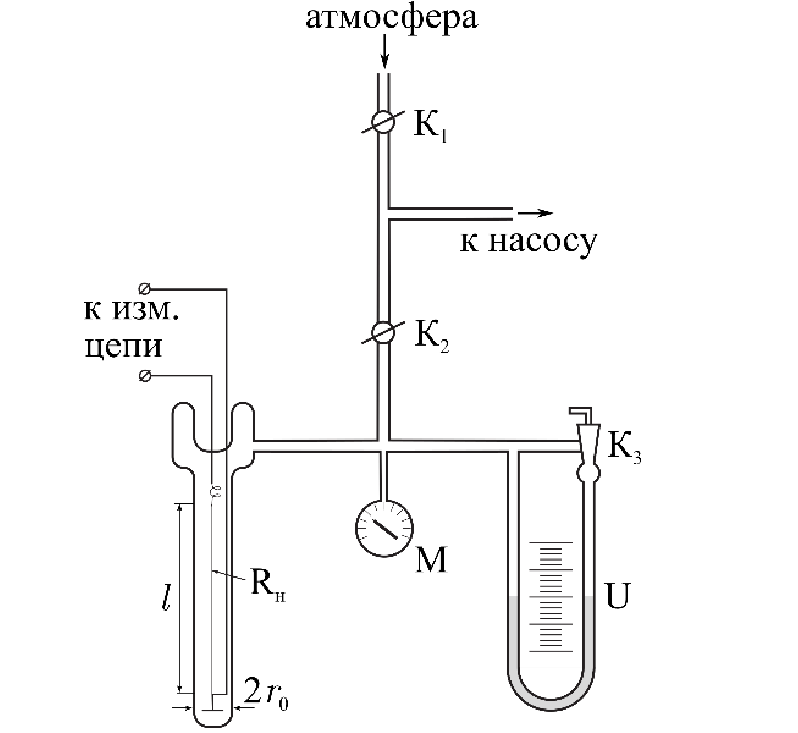
\includegraphics[width=0.4\linewidth]{vacuum.png}
            \caption{Вакуумная часть экспериментальной установки}
            \label{vacuum_part}
        \end{figure}
        Вакуумная установка состоит из форвакуумного насоса, стрелочного вакуумметра $M$ и U-образного масляного манометра. Вакуумметр служит для
        измерения высоких давлений вплоть до $\sim 10 \text{торр}$ (он показывает разность
        давлений между установкой и атмосферой, так что нуль на его шкале соответствует атмосферному давлению в установке). U-образный манометр 
        заполнен маслом с плотностью $\rho_{\text{м}} = 0.885 \text{г}/\text{см}^3$ и предназначен для измерения
        низких давлений (вплоть до $\sim 0.1 \text{торр}$). Кран К1 служит для соединения установки и насоса с атмосферой, кран К2 — для отсоединения откачиваемого
        объёма от насоса, кран К3 — для соединения колен U-образного манометра.\\
        Металлическая нить служит как источником тепла, так и датчиком темпера-
        туры (термометром сопротивления). В рабочем диапазоне температур ($20–40 \circ C$)
        сопротивление платины зависит от температуры практически линейно:
        \begin{equation}\label{sopr}
            R(t) = R_0(1+\alpha t)
        \end{equation}
        где $t$ - температура в $[\circ C]$, $R_0$ - сопротивление при $0 \circ C$, и 
        \[
            \alpha_0 = \frac{1}{R_0}\frac{dR}{dt} = 3.92\cdot 10^{-3} \circ C^-1   
        \]
        -температурный коэффициент сопротивления пластины в указанном диапазоне.
        \begin{figure}[H]
            \centering
            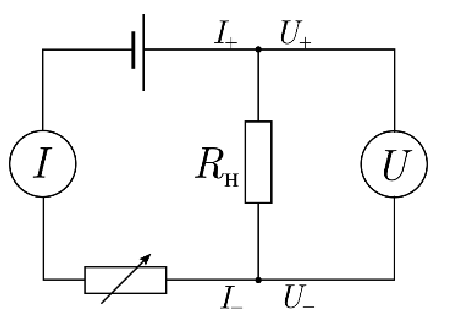
\includegraphics[width=0.4\linewidth]{electricity.png}
            \caption{Электическая схема измерений}
            \label{electricity}
        \end{figure}
        Электрическая схема установки приведена на \ref{electricity} Для измерения сопротивления нити $R_{\text{н}}$ 
        используется четырёхпроводная схема. По двум проводам (токовая пара $I_{+}$ и $I_{-}$) через сопротивление
        пропускается измерительный ток, а два других (потенциальная пара $U_{+}$ и $U_{-}$) используются
        для параллельного подключения вольтметра. Ток $I$ через сопротивление и напряжение $U$ на нём 
        измеряются цифровыми мультиметрами, один из которых работает в режиме амперметра, а другой — вольтметра. 
        Сопротивление находится по закону Ома: $R_{\text{н}} = U/I$. Те же измерения позволяют определить мощность 
        нагрева проволоки: $Q = UI$. Ток в цепи регулируется с помощью магазина сопротивлений, включённого 
        последовательно с источником тока. Для предотвращения перегорания нити в цепь включено дополнительное 
        сопротивление (10 Ом). Напряжение на источнике питания $2 B$

    
    \section{Ход работы}     
        \begin{enumerate}
            \item Проведем предварительные расчеты параметров опыта. Приняв газокинетический диаметр молекул равным $d \sim 3.5 A$, оценим
            длину свободного пробега молекул при атмосферном давлении.\\
            Оценим, при каком давлении $P_1$ длина свободного пробега сравняется с радиусом нити. В единицах масляного столба: $P_1 \approx 500 \text{мм.масл.ст.}$
            \item Запишем значения атмосферного давления $P_{\text{атм}}$ и температуры $t_{\text{к}}$ в комнате.
            \item Убедимся, что перед началом эксперимента установка находится под вакуумом. Кран $K_1$ открыт, $K_2$ — закрыт, $K_3$— открыт.
            \item Запустим воздух в установку, плавно открывая кран $K_2$, включим в сеть цифровые мультиметры. Установите амперметр в режим
            измерения постоянного тока, а вольтметр — постоянного напряжения.
            \item 
            
                    
        \end{enumerate}
    \section{Вывод}

\newpage
\section{Приложение 1}
\begin{table}[H]
\centering
\caption{$P = 69$ Па}
\begin{tabular}{rrllll}
\hline
 $U$, В &  $I$, мА &     $R$, Ом & $\Delta R$, Ом &     $Q$, мкВт & $\Delta Q$, мВт \\ \hline
0.178 & 15.722 & 11.32 &           0.06 &  2.80 &            0.02 \\ \hline
0.232 & 20.566 & 11.28 &           0.05 &  4.77 &            0.02 \\ \hline
0.342 & 30.126 & 11.35 &           0.03 & 10.30 &            0.03 \\ \hline
0.412 & 36.045 & 11.43 &           0.03 & 14.85 &            0.04 \\ \hline
0.542 & 46.911 & 11.55 &           0.02 & 25.43 &            0.05 \\ \hline
0.600 & 51.683 & 11.61 &           0.02 & 31.01 &            0.05 \\ \hline
0.822 & 68.858 & 11.94 &           0.01 & 56.60 &            0.07 \\ \hline
\end{tabular}
\end{table}
\begin{figure}[H]\centering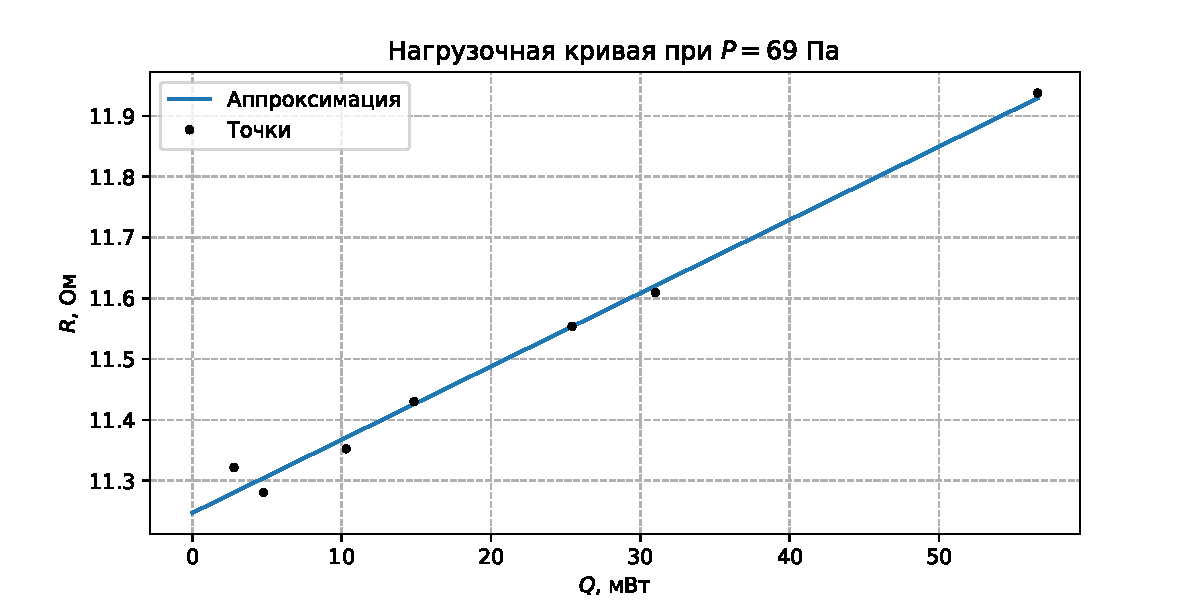
\includegraphics[width=\textwidth]{graphs/RQ69.45.pdf}\end{figure}\begin{table}[H]
\centering
\caption{$P = 83$ Па}
\begin{tabular}{rrllll}
\hline
 $U$, В &  $I$, мА &     $R$, Ом & $\Delta R$, Ом &     $Q$, мкВт & $\Delta Q$, мВт \\ \hline
0.126 & 11.172 & 11.28 &           0.09 &  1.41 &            0.01 \\ \hline
0.175 & 15.489 & 11.30 &           0.06 &  2.71 &            0.02 \\ \hline
0.293 & 25.863 & 11.33 &           0.04 &  7.58 &            0.03 \\ \hline
0.397 & 34.816 & 11.40 &           0.03 & 13.82 &            0.03 \\ \hline
0.482 & 42.084 & 11.45 &           0.02 & 20.28 &            0.04 \\ \hline
0.583 & 54.466 & 10.70 &           0.02 & 31.75 &            0.05 \\ \hline
0.670 & 57.587 & 11.63 &           0.02 & 38.58 &            0.06 \\ \hline
0.788 & 66.910 & 11.78 &           0.01 & 52.73 &            0.07 \\ \hline
\end{tabular}
\end{table}
\begin{figure}[H]\centering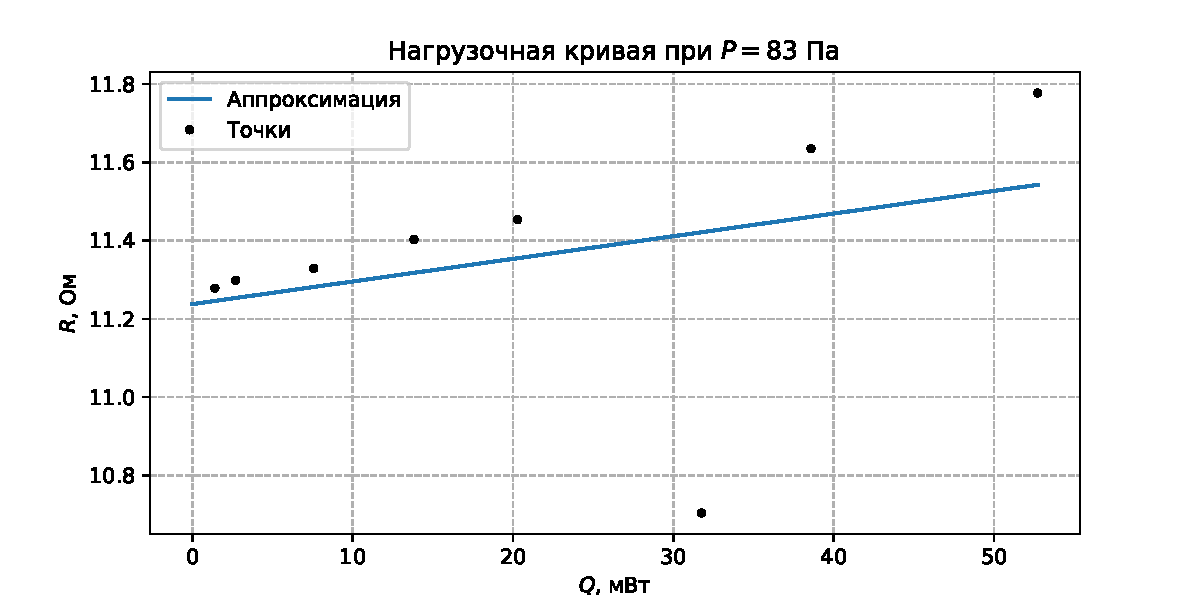
\includegraphics[width=\textwidth]{graphs/RQ83.0719363645837.pdf}\end{figure}\begin{table}[H]
\centering
\caption{$P = 103$ Па}
\begin{tabular}{rrllll}
\hline
 $U$, В &  $I$, мА &     $R$, Ом & $\Delta R$, Ом &     $Q$, мкВт & $\Delta Q$, мВт \\ \hline
0.121 & 10.636 & 11.38 &           0.09 &  1.29 &            0.01 \\ \hline
0.177 & 15.605 & 11.34 &           0.06 &  2.76 &            0.02 \\ \hline
0.291 & 25.548 & 11.39 &           0.04 &  7.43 &            0.03 \\ \hline
0.334 & 29.270 & 11.41 &           0.03 &  9.78 &            0.03 \\ \hline
0.391 & 34.266 & 11.41 &           0.03 & 13.40 &            0.03 \\ \hline
0.473 & 41.300 & 11.45 &           0.02 & 19.53 &            0.04 \\ \hline
0.598 & 51.935 & 11.51 &           0.02 & 31.06 &            0.05 \\ \hline
0.813 & 69.731 & 11.66 &           0.01 & 56.69 &            0.07 \\ \hline
\end{tabular}
\end{table}
\begin{figure}[H]\centering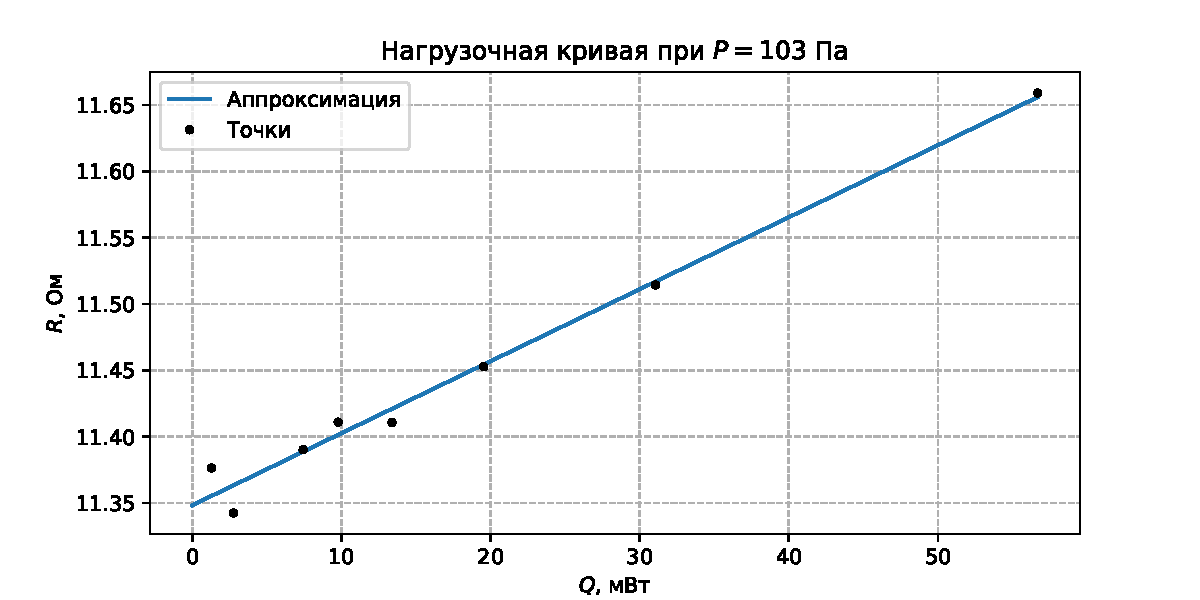
\includegraphics[width=\textwidth]{graphs/RQ103.34132342824749.pdf}\end{figure}\begin{table}[H]
\centering
\caption{$P = 137$ Па}
\begin{tabular}{rrllll}
\hline
 $U$, В &  $I$, мА &       $R$, Ом & $\Delta R$, Ом &    $Q$, мкВт & $\Delta Q$, мВт \\ \hline
    1 &      1 & 1000.00 &           1.41 & 1.00 &            0.00 \\ \hline
    2 &      2 & 1000.00 &           0.71 & 4.00 &            0.00 \\ \hline
    3 &      3 & 1000.00 &           0.47 & 9.00 &            0.00 \\ \hline
\end{tabular}
\end{table}
\begin{figure}[H]\centering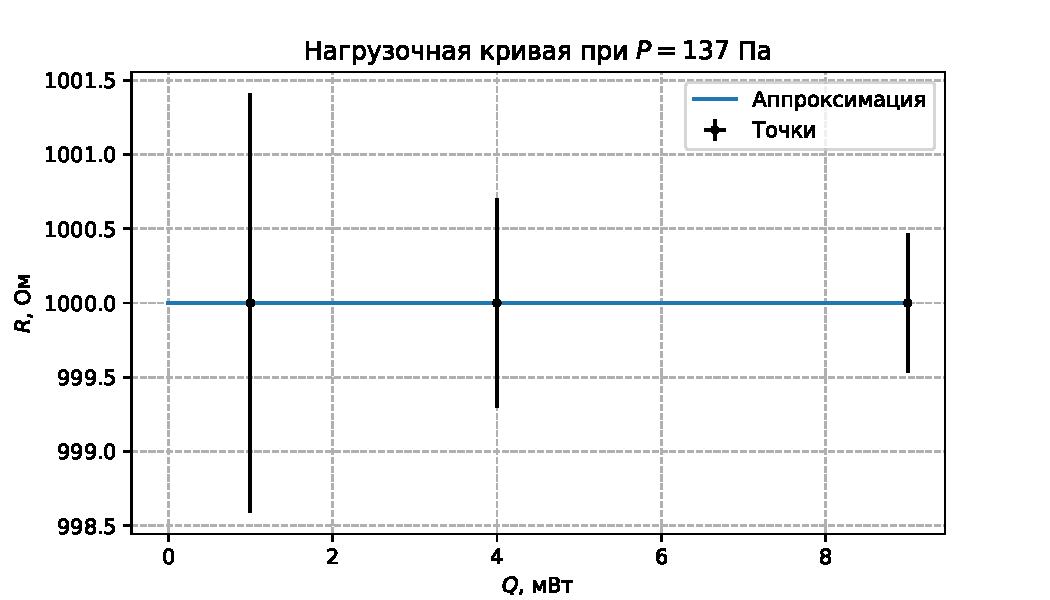
\includegraphics[width=\textwidth]{graphs/RQ136.694512232762.pdf}\end{figure}\begin{table}[H]
\centering
\caption{$P = 202$ Па}
\begin{tabular}{rrllll}
\hline
 $U$, В &  $I$, мА &     $R$, Ом & $\Delta R$, Ом &     $Q$, мкВт & $\Delta Q$, мВт \\ \hline
0.135 & 11.890 & 11.35 &           0.08 &  1.61 &            0.01 \\ \hline
0.243 & 21.432 & 11.34 &           0.05 &  5.21 &            0.02 \\ \hline
0.323 & 28.408 & 11.37 &           0.04 &  9.18 &            0.03 \\ \hline
0.377 & 33.095 & 11.39 &           0.03 & 12.48 &            0.03 \\ \hline
0.567 & 49.267 & 11.51 &           0.02 & 27.93 &            0.05 \\ \hline
0.732 & 63.060 & 11.61 &           0.02 & 46.16 &            0.06 \\ \hline
\end{tabular}
\end{table}
\begin{figure}[H]\centering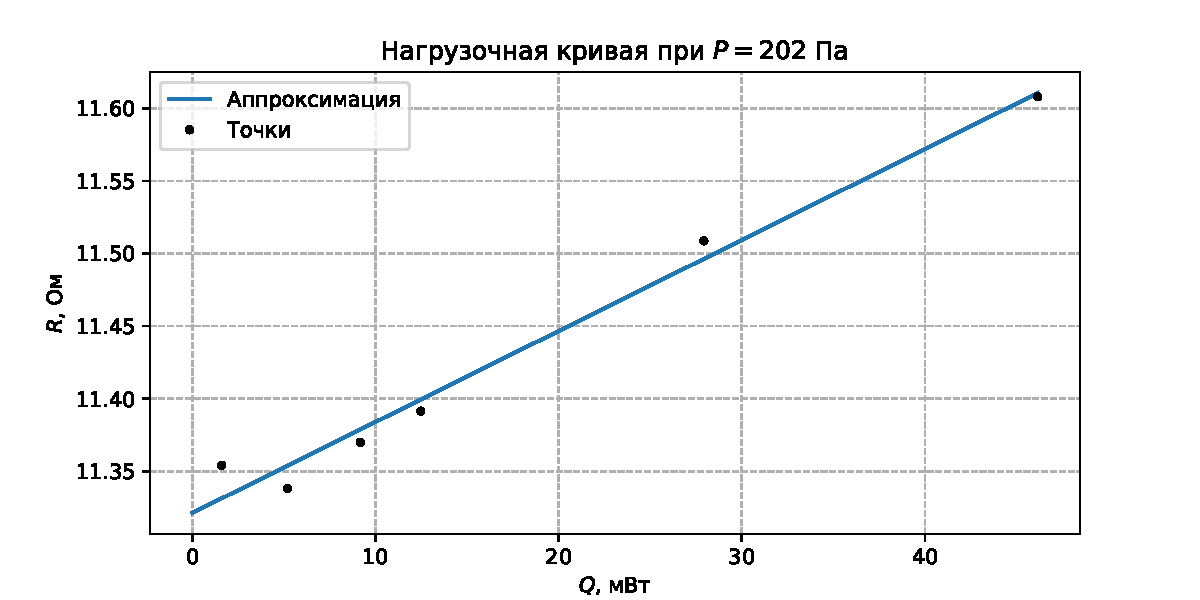
\includegraphics[width=\textwidth]{graphs/RQ201.83695244139577.pdf}\end{figure}\begin{table}[H]
\centering
\caption{$P = 386$ Па}
\begin{tabular}{rrllll}
\hline
 $U$, В &  $I$, мА &       $R$, Ом & $\Delta R$, Ом &    $Q$, мкВт & $\Delta Q$, мВт \\ \hline
    1 &      1 & 1000.00 &           1.41 & 1.00 &            0.00 \\ \hline
    2 &      2 & 1000.00 &           0.71 & 4.00 &            0.00 \\ \hline
    3 &      3 & 1000.00 &           0.47 & 9.00 &            0.00 \\ \hline
\end{tabular}
\end{table}
\begin{figure}[H]\centering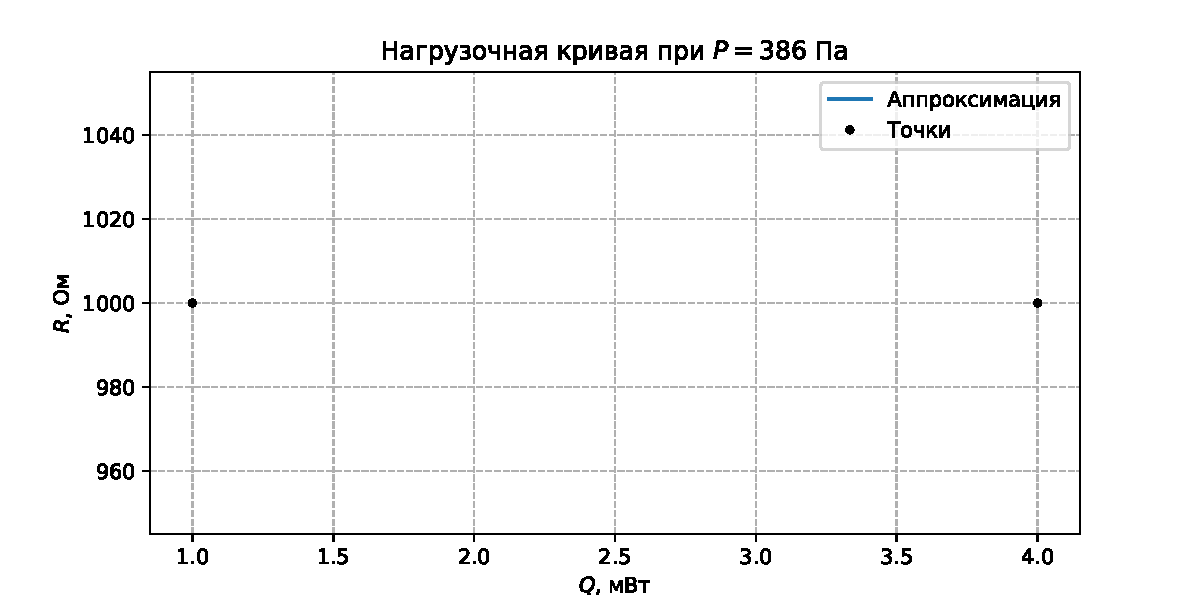
\includegraphics[width=\textwidth]{graphs/RQ385.5933585713642.pdf}\end{figure}\begin{table}[H]
\centering
\caption{$P = 4304$ Па}
\begin{tabular}{rrllll}
\hline
 $U$, В &  $I$, мА &     $R$, Ом & $\Delta R$, Ом &     $Q$, мкВт & $\Delta Q$, мВт \\ \hline
0.135 & 11.894 & 11.35 &           0.08 &  1.61 &            0.01 \\ \hline
0.290 & 25.519 & 11.36 &           0.04 &  7.40 &            0.03 \\ \hline
0.390 & 34.219 & 11.40 &           0.03 & 13.35 &            0.03 \\ \hline
0.472 & 41.231 & 11.45 &           0.02 & 19.46 &            0.04 \\ \hline
0.596 & 51.835 & 11.50 &           0.02 & 30.89 &            0.05 \\ \hline
0.781 & 67.299 & 11.60 &           0.01 & 52.56 &            0.07 \\ \hline
\end{tabular}
\end{table}
\begin{figure}[H]\centering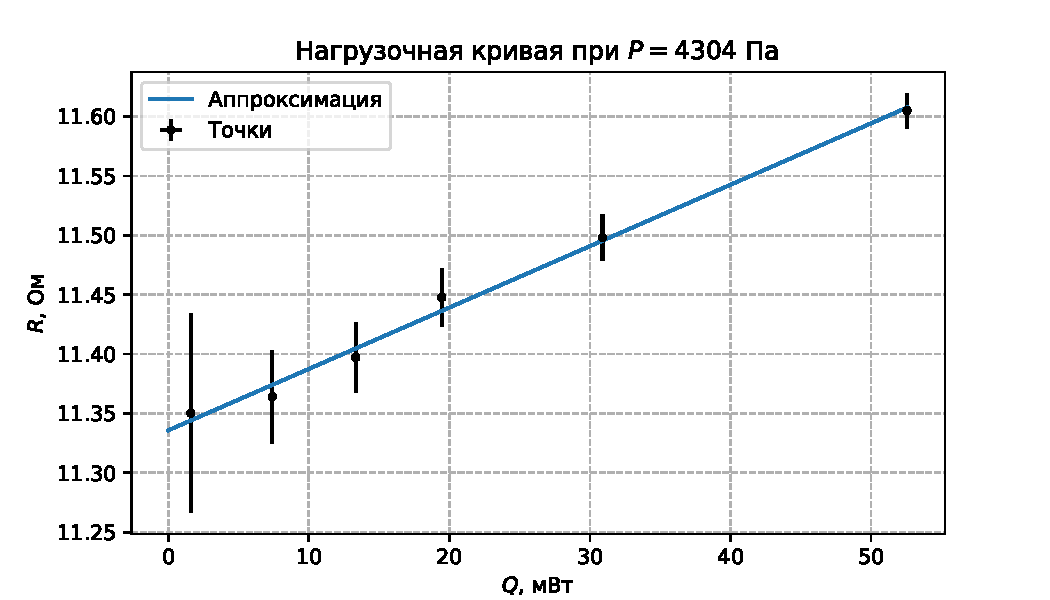
\includegraphics[width=\textwidth]{graphs/RQ4304.46.pdf}\end{figure}\begin{table}[H]
\centering
\caption{$P = 5658$ Па}
\begin{tabular}{rrllll}
\hline
 $U$, В &  $I$, мА &     $R$, Ом & $\Delta R$, Ом &     $Q$, мкВт & $\Delta Q$, мВт \\ \hline
0.164 & 14.463 & 11.34 &           0.07 &  2.37 &            0.01 \\ \hline
0.258 & 22.640 & 11.40 &           0.04 &  5.84 &            0.02 \\ \hline
0.390 & 34.216 & 11.40 &           0.03 & 13.34 &            0.03 \\ \hline
0.472 & 41.235 & 11.45 &           0.02 & 19.46 &            0.04 \\ \hline
0.597 & 51.824 & 11.52 &           0.02 & 30.94 &            0.05 \\ \hline
0.755 & 65.164 & 11.59 &           0.02 & 49.20 &            0.07 \\ \hline
\end{tabular}
\end{table}
\begin{figure}[H]\centering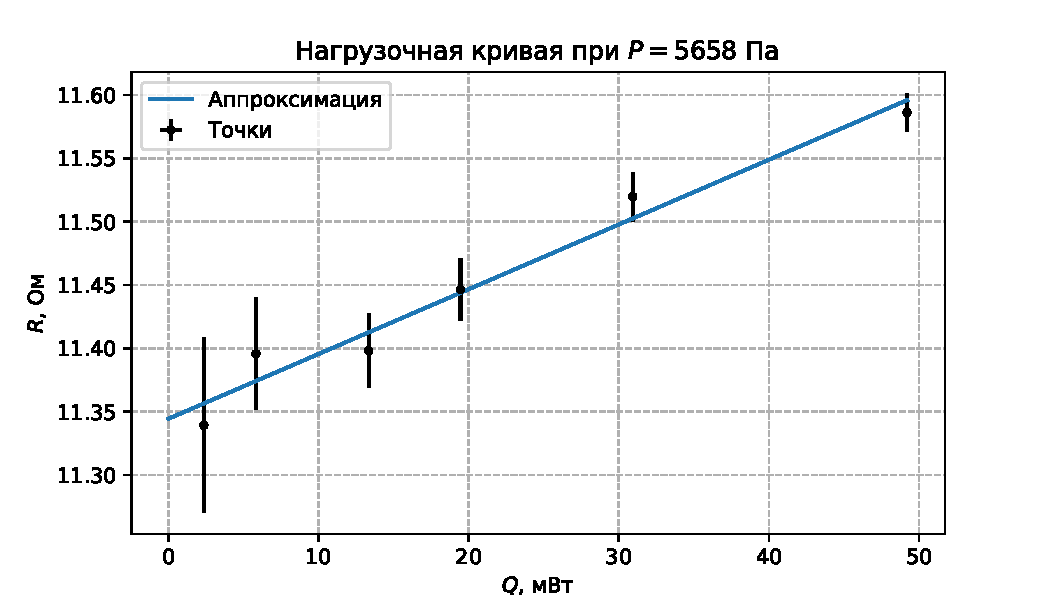
\includegraphics[width=\textwidth]{graphs/RQ5657.8637324185265.pdf}\end{figure}\begin{table}[H]
\centering
\caption{$P = 8253$ Па}
\begin{tabular}{rrllll}
\hline
 $U$, В &  $I$, мА &     $R$, Ом & $\Delta R$, Ом &     $Q$, мкВт & $\Delta Q$, мВт \\ \hline
0.165 & 14.580 & 11.32 &           0.07 &  2.41 &            0.01 \\ \hline
0.257 & 22.648 & 11.35 &           0.04 &  5.82 &            0.02 \\ \hline
0.389 & 34.245 & 11.36 &           0.03 & 13.32 &            0.03 \\ \hline
0.470 & 41.275 & 11.39 &           0.02 & 19.40 &            0.04 \\ \hline
0.594 & 51.906 & 11.44 &           0.02 & 30.83 &            0.05 \\ \hline
0.755 & 65.151 & 11.59 &           0.02 & 49.19 &            0.07 \\ \hline
\end{tabular}
\end{table}
\begin{figure}[H]\centering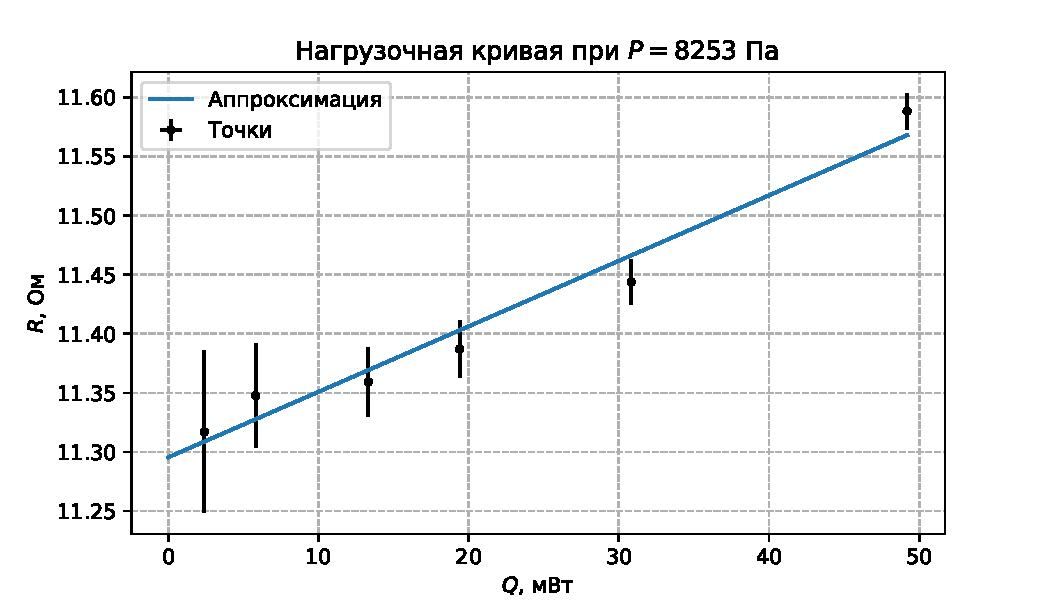
\includegraphics[width=\textwidth]{graphs/RQ8252.654613598917.pdf}\end{figure}\begin{table}[H]
\centering
\caption{$P = 15244$ Па}
\begin{tabular}{rrllll}
\hline
 $U$, В &  $I$, мА &     $R$, Ом & $\Delta R$, Ом &     $Q$, мкВт & $\Delta Q$, мВт \\ \hline
0.178 & 15.704 & 11.33 &           0.06 &  2.80 &            0.02 \\ \hline
0.260 & 22.872 & 11.37 &           0.04 &  5.95 &            0.02 \\ \hline
0.337 & 29.630 & 11.37 &           0.03 &  9.99 &            0.03 \\ \hline
0.480 & 42.025 & 11.42 &           0.02 & 20.17 &            0.04 \\ \hline
0.610 & 53.086 & 11.49 &           0.02 & 32.38 &            0.05 \\ \hline
0.779 & 67.050 & 11.62 &           0.01 & 52.23 &            0.07 \\ \hline
\end{tabular}
\end{table}
\begin{figure}[H]\centering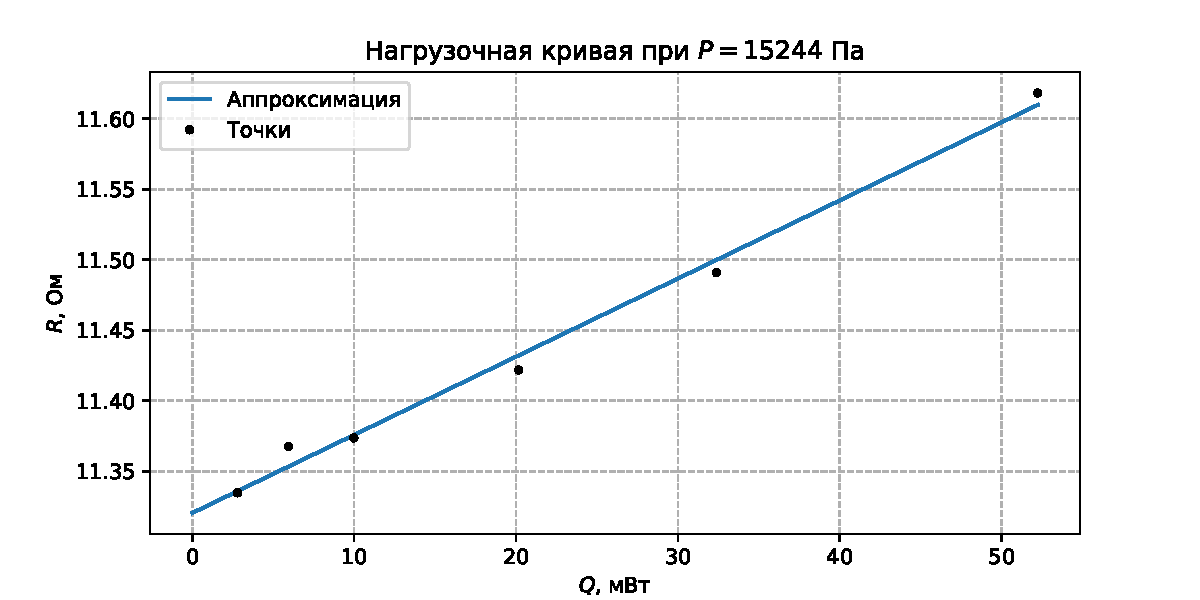
\includegraphics[width=\textwidth]{graphs/RQ15243.64502645898.pdf}\end{figure}\begin{table}[H]
\centering
\caption{$P = 99710$ Па}
\begin{tabular}{rrllll}
\hline
 $U$, В &  $I$, мА &     $R$, Ом & $\Delta R$, Ом &     $Q$, мкВт & $\Delta Q$, мВт \\ \hline
0.121 & 10.636 & 11.38 &           0.09 &  1.29 &            0.01 \\ \hline
0.177 & 15.605 & 11.34 &           0.06 &  2.76 &            0.02 \\ \hline
0.291 & 25.548 & 11.39 &           0.04 &  7.43 &            0.03 \\ \hline
0.334 & 29.270 & 11.41 &           0.03 &  9.78 &            0.03 \\ \hline
0.391 & 34.266 & 11.41 &           0.03 & 13.40 &            0.03 \\ \hline
0.473 & 41.300 & 11.45 &           0.02 & 19.53 &            0.04 \\ \hline
0.598 & 51.935 & 11.51 &           0.02 & 31.06 &            0.05 \\ \hline
0.813 & 69.731 & 11.66 &           0.01 & 56.69 &            0.07 \\ \hline
\end{tabular}
\end{table}
\begin{figure}[H]\centering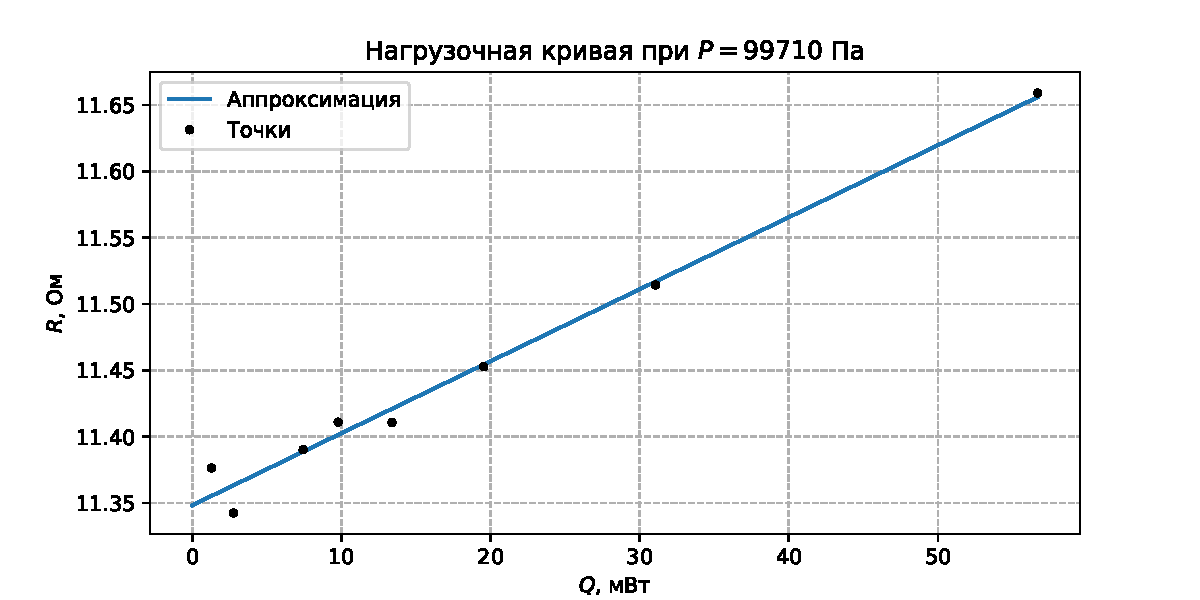
\includegraphics[width=\textwidth]{graphs/RQ99710.0.pdf}\end{figure}

\end{document}
